Due to the large offsets and parallax between the camera and projector, the project shifts its focus from physical testing to software testing and real-time performance analysis. Following the details on implementation in Section \ref{implementation}, this section aims to describe the testing process for testing both the system and the toolsets, including an evaluation of the backscatter cancellation system performance.

\subsection{Bubble Backscatter Simulator}

The bubble backscatter simulator program works very well as a simple backscatter simulation. As Figure \ref{fig:sim_validate} illustrates, the program successfully renders a preview graphical user interface, enabling the user to view the bubbles as they generate and move, and the program also correctly exports each frame of the simulation as a PNG file, emulating the frame-by-frame capture loop behaviour of the backscatter cancellation system. Furthermore, the program exports a CSV dataset of the individual backscatter particle positions and radii from each frame, classing each particle with a unique ID, for the first few particles in the dataset. Despite this, a major drawback that I found from this program is the fact that it doesn't simulate varying backscatter appearances, such as morphological transformations with shape warping, and colour changes, to verify if the system can detect varying backscatter parameters, as all particles are exactly circular and white. In addition, the program does not simulate varying background conditions as the background is exactly black, resulting in the inability to verify whether the system can correctly isolate and segment just the particles and not any regions of interest in the background.

\begin{figure}[H]
    \centering
    \begin{subfigure}{.49\textwidth}
        \centering
        \includegraphics[width=1\linewidth]{assets/test-sim-sc.png}
        \caption{}
        \label{fig:sim_sc}
    \end{subfigure}
    \hfill
    \begin{subfigure}{.49\textwidth}
        \centering
        \includegraphics[width=1\linewidth]{assets/test-sim-frames.png}
        \caption{}
        \label{fig:sim_frames}
    \end{subfigure}
    \caption{Screenshots validating the Bubble Backscatter Simulator program: (\ref{sub@fig:sim_sc}) showing the preview GUI window, and (\ref{sub@fig:sim_frames}) showing the list of frames in the output directory.}
    \label{fig:sim_validate}
\end{figure}

\subsection{Lossless Video Recorder}
The lossless video recorder proved an invaluable tool that performed almost flawlessly, as Figure \ref{fig:rec_validate} illustrates. A change I had to make was to modify the OS to ensure the console would not output to the HDMI Framebuffer, as this was causing interference with my Framebuffer-driven light source. Unfortunately, as the figure also illustrates, there was a major misalignment issue, where the camera is only able to a small corner in the bottom-left of the projector-lit scene. While a simple cropping function can resolve most of this, which I have implemented in the backscatter cancellation system, albeit reducing the system's useable region, the system will still be affected by the camera's internal reflection, which reduces the field of view and adds distortion. Nevertheless, the recordings were very helpful in verifying the system in a non-synthetic environment without requiring re-deployment underwater.

\begin{figure}[H]
    \centering
    \begin{subfigure}{.49\textwidth}
        \centering
        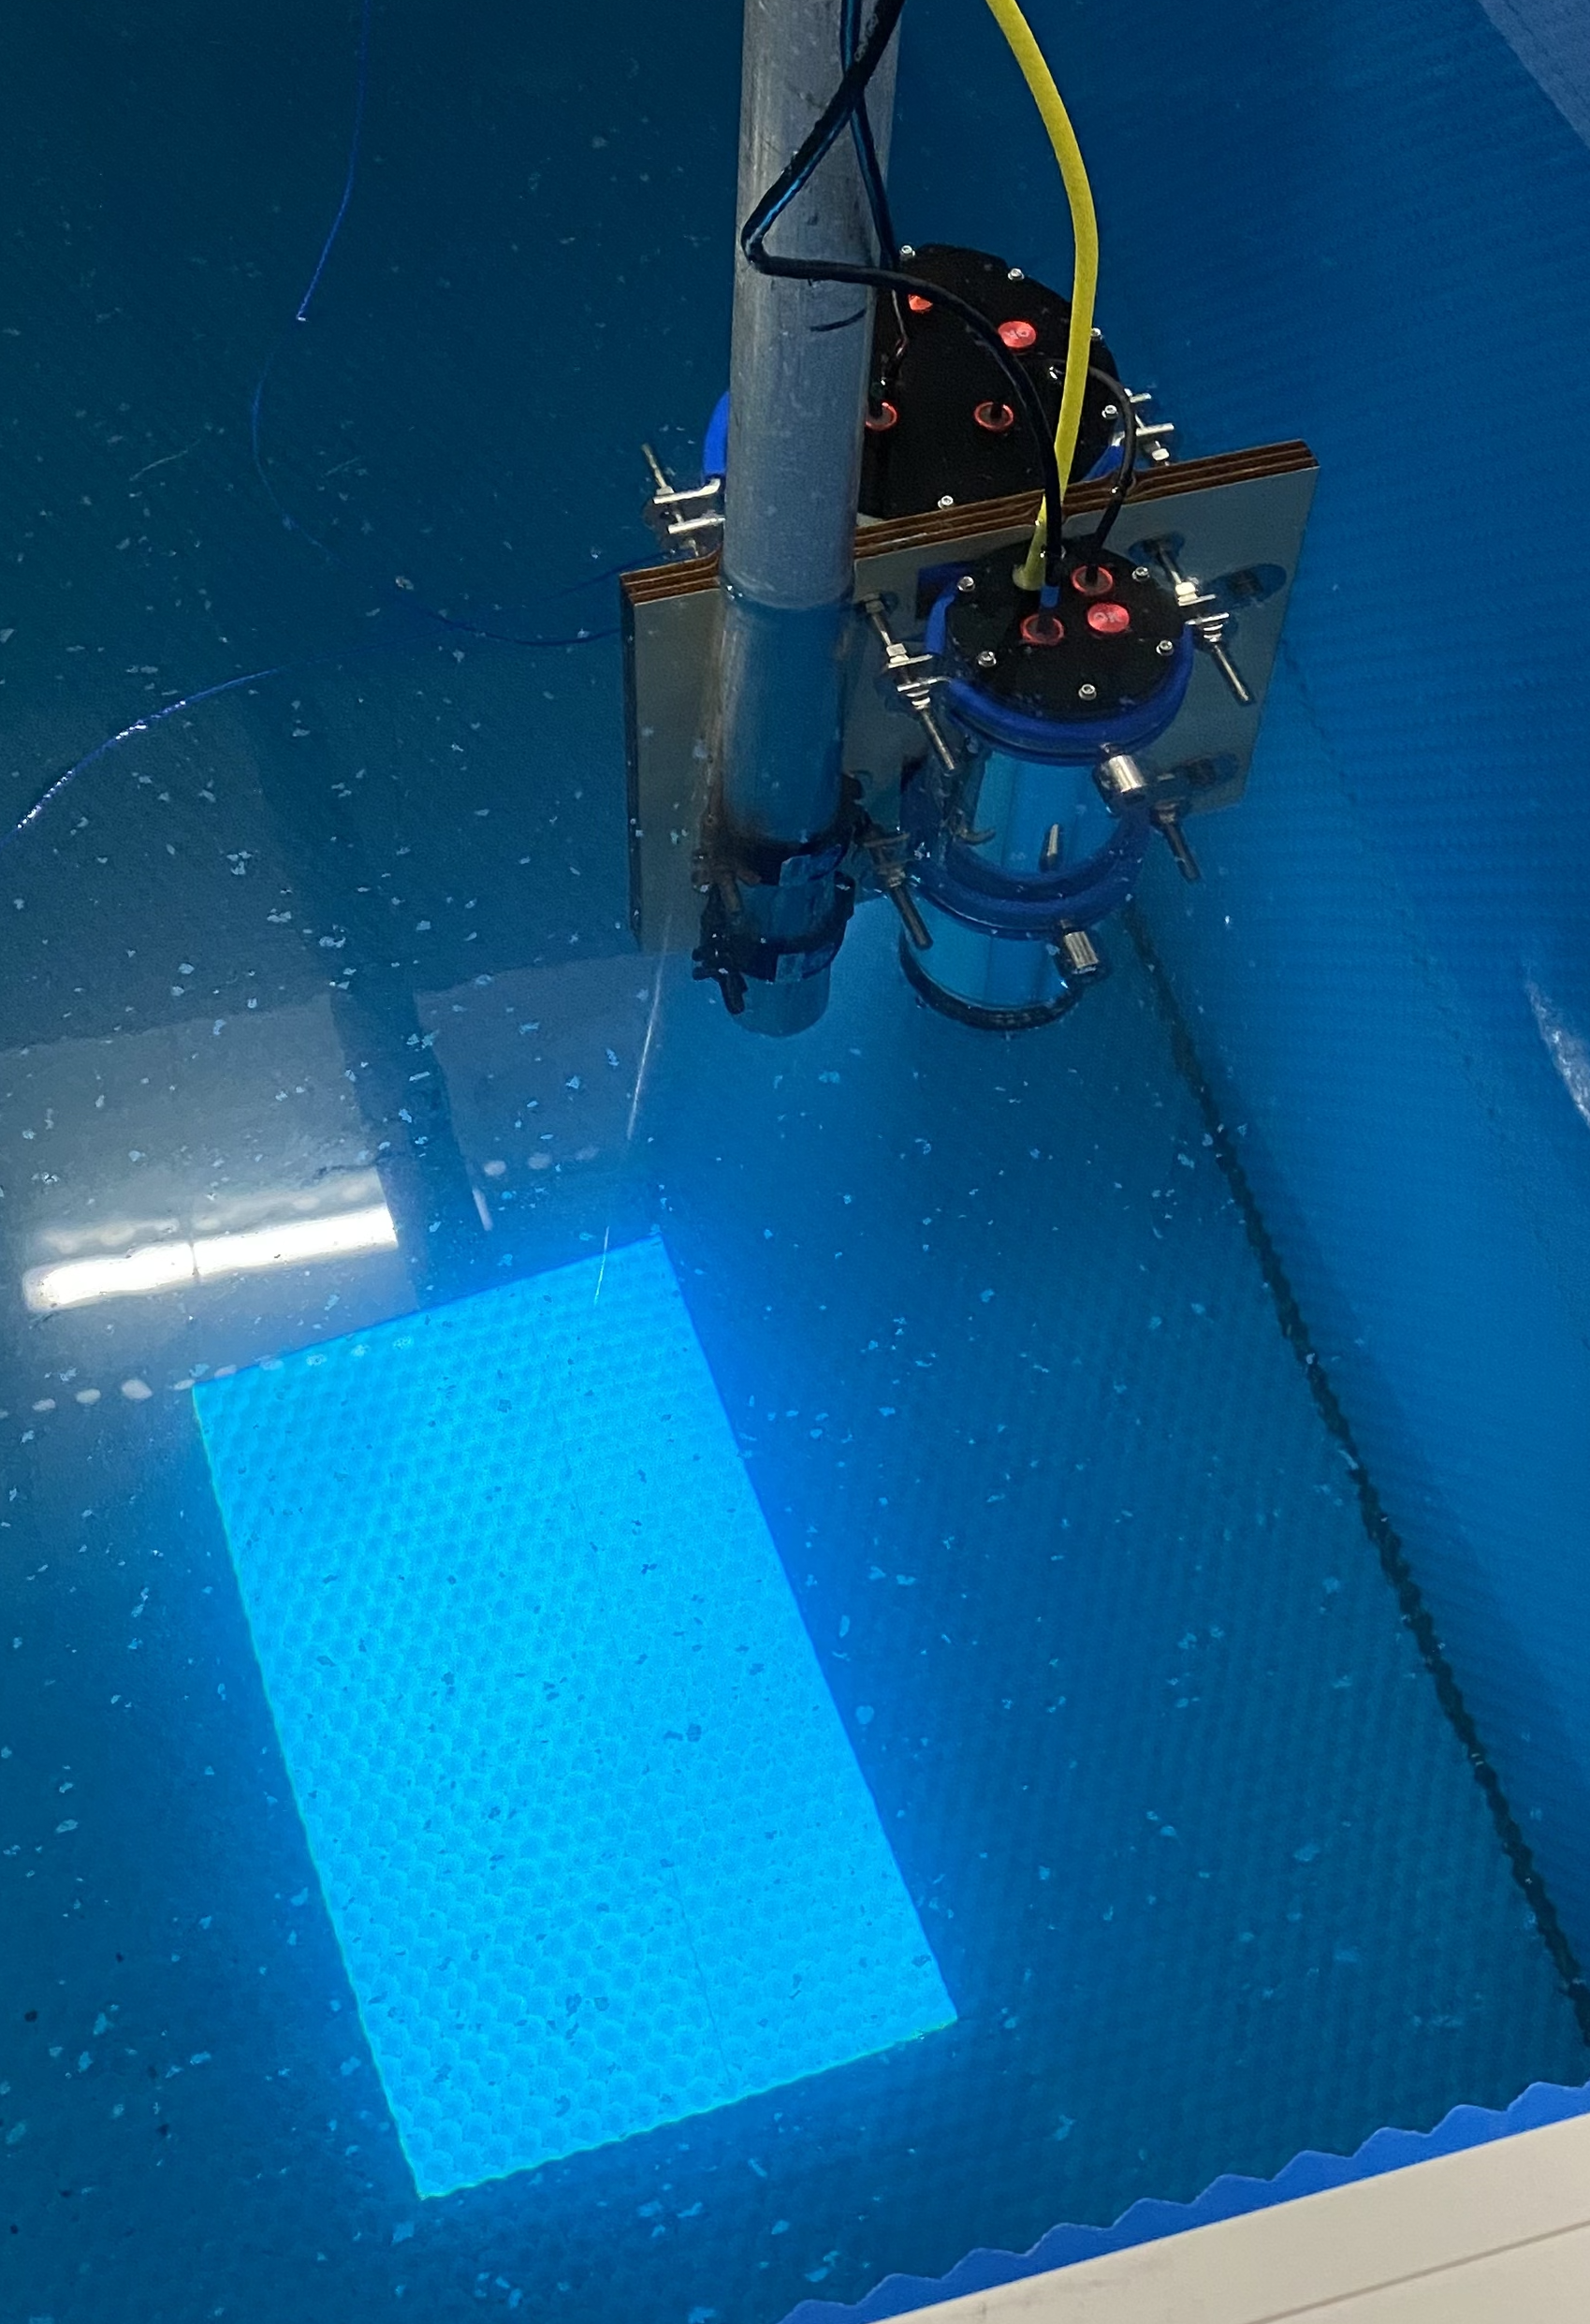
\includegraphics[width=1\linewidth]{assets/underwater-testing.png}
        \caption{}
        \label{fig:underwater}
    \end{subfigure}
    \hfill
    \begin{subfigure}{.49\textwidth}
        \centering
        \begin{subfigure}{\textwidth}
            \centering
            \includegraphics[width=1\linewidth]{assets/rec-frame.png}
            \caption{}
            \label{fig:rec_frame}
        \end{subfigure}
        \vfill
        \begin{subfigure}{\textwidth}
            \centering
            \includegraphics[width=1\linewidth]{assets/rec_sc.png}
            \caption{}
            \label{fig:rec_sc}
        \end{subfigure}
    \end{subfigure}
    \caption{Figures validating the Lossless Video Recorder program: (\subref{fig:underwater}) showing the submersible recording underwater at the Institute for Safe Autonomy testing tank, (\subref{fig:rec_frame}) an extracted frame from recorded footage, and (\subref{fig:rec_sc}) showing the preview GUI window, rendered remotely with X11 forwarding.}
    \label{fig:rec_validate}
\end{figure}

\subsection{Backscatter Cancellation System}
I first verified the backscatter cancellation system using the output from the backscatter simulation and it worked flawlessly, identifying and segmenting the bubbles correctly using the minimum enclosing circle logic, as Figure \ref{fig:sys_sim} illustrates. However, when using the underwater test footage, the system started to incorrectly detect the background, mainly the textured padding of the testing tank, as Figure \ref{fig:sys_histequ} illustrates. I identified that this was caused by the histogram equalisation stage, where the entire image frame's pixel intensities are spread, increasing the contrast substantially. I therefore replaced this stage with an OpenCV binary thresholding implementation, ensuring that the system only passes certain pixel intensities. The results after this processing pipeline stage replacement were much better, as Figure \ref{fig:sys_binth} illustrates. Figure \ref{fig:sys_flow_visual} illustrates the final system's image processing pipeline flow.

\begin{figure}[H]
    \centering
    \begin{subfigure}{.48\textwidth}
        \centering
        \includegraphics[width=1\linewidth]{assets/sys_sim.png}
        \caption{}
        \label{fig:sys_sim}
    \end{subfigure}
    \hfill
    \begin{subfigure}{.25\textwidth}
        \centering
        \includegraphics[width=1\linewidth]{assets/sys_histequ.png}
        \caption{}
        \label{fig:sys_histequ}
    \end{subfigure}
    \hfill
    \begin{subfigure}{.25\textwidth}
        \centering
        \includegraphics[width=1\linewidth]{assets/sys_binth.png}
        \caption{}
        \label{fig:sys_binth}
    \end{subfigure}
    \caption{Screenshots validating the Backscatter Cancellation System program: (\ref{sub@fig:sys_sim}) showing the backscatter segmentation (red circles) from the Backscatter Simulator output, (\ref{sub@fig:sys_histequ}) incorrect segmentation of backscatter from the test footage, and (\ref{sub@fig:sys_binth}), which shows the correct backscatter segmentation using the same footage.}
    \label{fig:sys_validate}
\end{figure}

\begin{figure}[H]
    \centering
    \begin{subfigure}{.6\textwidth}
        \begin{subfigure}{0.32\textwidth}
            \centering
            \includegraphics[width=1\linewidth]{assets/sys_input.png}
            \caption{}
            \label{fig:sys_input}
        \end{subfigure}
        \hfill
        \begin{subfigure}{0.32\textwidth}
            \centering
            \includegraphics[width=1\linewidth]{assets/sys_gs.png}
            \caption{}
            \label{fig:sys_gs}
        \end{subfigure}
        \hfill
        \begin{subfigure}{0.32\textwidth}
            \centering
            \includegraphics[width=1\linewidth]{assets/sys_gb.png}
            \caption{}
            \label{fig:sys_gb}
        \end{subfigure}
        \hfill
        \begin{subfigure}{0.32\textwidth}
            \centering
            \includegraphics[width=1\linewidth]{assets/sys_thresh.png}
            \caption{}
            \label{fig:sys_thresh}
        \end{subfigure}
        \hfill
        \begin{subfigure}{0.32\textwidth}
            \centering
            \includegraphics[width=1\linewidth]{assets/sys_canny.png}
            \caption{}
            \label{fig:sys_canny}
        \end{subfigure}
        \hfill
        \begin{subfigure}{0.32\textwidth}
            \centering
            \includegraphics[width=1\linewidth]{assets/sys_segment.png}
            \caption{}
            \label{fig:sys_segment}
        \end{subfigure}
    \end{subfigure}
    \hfill
    \begin{subfigure}{.39\textwidth}
        \centering
        \includegraphics[width=1\linewidth]{assets/sys_project.png}
        \caption{}
        \label{fig:sys_projection}
    \end{subfigure}
    \caption{Screenshots previewing the image processing pipeline stages of the Cancellation System program, in order from left to right: (\ref{sub@fig:sys_input}) the input, (\ref{sub@fig:sys_gs}) greyscale filtering, (\ref{sub@fig:sys_gb}) Gaussian blur, (\ref{sub@fig:sys_thresh}) binary thresholding, (\ref{sub@fig:sys_canny}) the Canny algorithm, (\ref{sub@fig:sys_segment}) segmentation with minimum enclosing circles, finally, (\ref{sub@fig:sys_projection}), the projection.}
    \label{fig:sys_flow_visual}
\end{figure}

\subsection{System Performance Evaluation}

Due to time constraints, I couldn't implement logic in the backscatter cancellation system which exports a dataset of detected backscatter particles, which I could've then used to compare with the simulation export, the synthetic ground truth, to quantify the accuracy performance of the system. Therefore, this section entirely focuses on the real-time performance, by analysing the execution time for each image processing pipeline, and the total execution time for each frame with the underwater testing tank footage input to the RPi SBC system with the system software `nice' value set to the lowest value (-20), ensuring the highest process priority, ultimately quantifying the impact of multiprocessing and the PREEMPT-RT kernel patch.

\begin{table}[H]
    \centering
    \begin{tabularx}{\linewidth}{c || X | X | X | X || X | X | X | X}
        \hline
        \multirow[c]{2}{*}{\textbf{Process}} & \multicolumn{4}{c||}{\textbf{Avg. Duration (\textbf{\textmu s})}} & \multicolumn{4}{c}{\textbf{Std. Deviation (\textbf{\textmu s})}}\\
        \cline{2-9}
         & \scriptsize{Std, SP} & \scriptsize{RT, SP} & \scriptsize{Std, MP} & \scriptsize{RT, MP} & \scriptsize{Std, SP} & \scriptsize{RT, SP} & \scriptsize{Std, MP} & \scriptsize{RT, MP} \\
        \hline
        \hline
        Frame Capture & 1,480 & 20,100 & 12,120 & 27,730 & 3199 & 9629 & 14990 & 11600 \\
        \hline
        Greyscale Filter & 193.4 & 2370 & 220.2 & 212.0 & 31.19 & 57.67 & 91.02 & 80.16 \\
        \hline
        Gaussian Blur & 159.2 & 319.2 & 339.5 & 378.8 & 148.2 & 457.4 & 653.0 & 599.0 \\
        \hline
        Binary Threshold & 19.79 & 29.70 & 64.10 & 81.34 & 5.144 & 61.15 & 57.45 & 111.3 \\
        \hline
        Canny Algorithm & 601.9 & 795.3 & 879.20 & 975.3 & 95.46 & 550.3 & 724.4 & 1427 \\
        \hline
        Find Contours & 110.8 & 135.8 & 180.0 & 252.2 & 43.16 & 184.2 & 134.0 & 389.2 \\
        \hline
        Find MECs & 41.88 & 47.14 & 45.60 & 47.05 & 30.84 & 36.67 & 92.65 & 41.89 \\
        \hline
        \hline
        \textbf{Tot. Duration (\textbf{\textmu s})} & 2,607 & 21,620 & 13,850 & 29,670 & 3253 & 9732 & 15140 & 11920 \\
        \hline
    \end{tabularx}
    \caption{Real-time system metrics using the standard (Std) and real-time (RT) kernel, in single-core (SP), and with multiprocessing (MP). Values rounded to the nearest 4 sig. figs.}
    \label{table:sys_std_sp_metrics}
\end{table}

Table \ref{table:sys_std_sp_metrics} transcribes the real-time metrics for the system, across 402 frames of real test footage recorded from the testing tank, listing the execution duration for all the image processing pipeline stages using the standard kernel, real-time kernel, multiprocessing, and in the standard single core mode under the GIL. The data shows a 431\% increase in total latency from the single-core to the multi-core program with the standard kernel, and 37\& increase of that in the real-time kernel, a 729\% increase when moving from the standard to the real-time kernel with single-core, and a 114\% increase when moving from that in the multiprocessing system. The data also contains the standard deviation of the individual processing stage and total system latencies to measure data variability, showing a 199\% increase in fluctuations when moving from the standard to real-time kernel in the single-code environment, and a 21\% decrease of that in the multiprocessing environment.

In contrast to the theory that previous sections cover regarding the reduction of latency with multiprocessing and a real-time OS, the data illustrates the complete opposite. The multiprocessing system employs queues, a form of Inter-Process Communication (IPC), to preserve data whilst processing asynchronously across multiple processes. These IPCs introduce vast computational overhead due to data serialisation and deserialisation when transmitting across processes and during OS context switching. Furthermore, while multiprocessing offers parallelism, it still cannot overcome the synchronous nature of I/O-bound processes, as the data quantifies showing a 719\% increase in frame capture durations between the standard single-core and standard multiprocessing systems. The PREEMPT-RT patch should've reduced system latency or at least resulted in more constant latency measurements. However, the data illustrates the patch increasing the frequency of preemption points in the kernel, resulting in more context switches, and when paired with the IPCs, slowing down the system rate and increasing latency.

To conclude, my single-core RPi SBC system achieves a total processing latency of just \SI{2.6}{\milli\second}, a great improvement from the system in De Charette et al., which takes \SI{4.1}{\milli\second} to process frames on a much more powerful desktop computer, and achieving the \SI{33.33}{\milli\second} (30FPS) target.
